\documentclass{beamer}

%
% Choose how your presentation looks.
%
% For more themes, color themes and font themes, see:
% http://deic.uab.es/~iblanes/beamer_gallery/index_by_theme.html
%
\mode<presentation>
{
  \usetheme{default}      % or try Darmstadt, Madrid, Warsaw, ...
  \usecolortheme{default} % or try albatross, beaver, crane, ...
  \usefonttheme{default}  % or try serif, structurebold, ...
  \setbeamertemplate{navigation symbols}{}
  \setbeamertemplate{caption}[numbered]
  \setbeamertemplate{footline}[page number]
  \setbeamercolor{frametitle}{fg=white}
  \setbeamercolor{footline}{fg=black}
} 

\usepackage[english]{babel}
\usepackage[utf8x]{inputenc}
\usepackage{tikz}
\usepackage{listings}
\usepackage{courier}
\usepackage{minted}
\usepackage{array}

\xdefinecolor{darkblue}{rgb}{0.1,0.1,0.7}
\xdefinecolor{dianablue}{rgb}{0.18,0.24,0.31}
\definecolor{commentgreen}{rgb}{0,0.6,0}
\definecolor{stringmauve}{rgb}{0.58,0,0.82}

\lstset{ %
  backgroundcolor=\color{white},      % choose the background color
  basicstyle=\ttfamily\small,         % size of fonts used for the code
  breaklines=true,                    % automatic line breaking only at whitespace
  captionpos=b,                       % sets the caption-position to bottom
  commentstyle=\color{commentgreen},  % comment style
  escapeinside={\%*}{*)},             % if you want to add LaTeX within your code
  keywordstyle=\color{blue},          % keyword style
  stringstyle=\color{stringmauve},    % string literal style
  showstringspaces=false,
  showlines=true
}

\lstdefinelanguage{scala}{
  morekeywords={abstract,case,catch,class,def,%
    do,else,extends,false,final,finally,%
    for,if,implicit,import,match,mixin,%
    new,null,object,override,package,%
    private,protected,requires,return,sealed,%
    super,this,throw,trait,true,try,%
    type,val,var,while,with,yield},
  otherkeywords={=>,<-,<\%,<:,>:,\#,@},
  sensitive=true,
  morecomment=[l]{//},
  morecomment=[n]{/*}{*/},
  morestring=[b]",
  morestring=[b]',
  morestring=[b]"""
}

\title[2016-11-10-lucaetal-root4j]{Reading ROOT data in Java and Spark}
\author{Jim Pivarski \and Viktor Khristenko}
\institute{Princeton/DIANA-HEP \and University of Iowa}
\date{November 11, 2016}

\begin{document}

\logo{\pgfputat{\pgfxy(0.11, 8)}{\pgfbox[right,base]{\tikz{\filldraw[fill=dianablue, draw=none] (0 cm, 0 cm) rectangle (50 cm, 1 cm);}}}\pgfputat{\pgfxy(0.11, -0.6)}{\pgfbox[right,base]{\tikz{\filldraw[fill=dianablue, draw=none] (0 cm, 0 cm) rectangle (50 cm, 1 cm);}
\includegraphics[height=0.99 cm]{diana-hep-logo.png}\tikz{\filldraw[fill=dianablue, draw=none] (0 cm, 0 cm) rectangle (4.9 cm, 1 cm);}}}}

\begin{frame}
  \titlepage
\end{frame}

\logo{\pgfputat{\pgfxy(0.11, 8)}{\pgfbox[right,base]{\tikz{\filldraw[fill=dianablue, draw=none] (0 cm, 0 cm) rectangle (50 cm, 1 cm);}
\includegraphics[height=1 cm]{diana-hep-logo.png}}}}

% Uncomment these lines for an automatically generated outline.
%\begin{frame}{Outline}
%  \tableofcontents
%\end{frame}

\begin{frame}{Background}
\textcolor{darkblue}{Several methods have been attempted:}

\begin{enumerate}
\item Convert all data from ROOT to another format (Avro).

\textcolor{gray}{$\rightarrow$ Two copies of all data.}

\textcolor{gray}{$\rightarrow$} \textcolor{gray}{Used by 2016 CMS dark matter analysis: Oliver Gutsche,}

\textcolor{white}{$\rightarrow$} \textcolor{gray}{Matteo Cremonesi, Cristina Mantilla.}

\item<2-> Access ROOT inside the JVM via JNI.

\textcolor{gray}{$\rightarrow$ Hard-to-diagnose segmentation faults.}

\item<3-> Access ROOT as an external process (pipe or socket).

\textcolor{gray}{$\rightarrow$ Fragile, and all data passes through text.}

\item<4-> Run PyROOT in PySpark.

\textcolor{gray}{$\rightarrow$ All data passes through text (PySpark uses a socket).}

\end{enumerate}
\end{frame}

\begin{frame}{A better way}

{\Large Read ROOT files directly in pure Java!}

\begin{itemize}
\item Only one copy of the data.
\item No fragile pipes, sockets, or JNI.
\item No performance loss to unnecessarily serializing data.
\item No need to install binary executables across the system: just pass the Maven Central coordinates to {\tt --packages}.
\end{itemize}

\vspace{0.5 cm}
\textcolor{gray}{(Ha, ha--- funny story: I knew about such a package and didn't think it would work for us. Revisited it, and it works very well.)}
\end{frame}

\begin{frame}{Comparison to Enric \& Danilo's solution}
\vspace{0.25 cm}
\begin{center}
\textcolor{darkblue}{\Large Solutions to different problems}

\vspace{0.25 cm}
\begin{tabular}{>{\centering}p{0.45\linewidth} | >{\centering\arraybackslash}p{0.45\linewidth}}
Viktor \& Jim & Enric \& Danilo \\\hline
Read ROOT files, perform calculations in Spark. & Spark launches and controls ROOT process. \\
\uncover<2->{User writes Spark/PySpark scripts on DataFrames.} & \uncover<2->{User writes C++ for each data partition.} \\
\uncover<3->{Good for using Spark features: caching, MLLib, third-party libraries connecting to Spark.} & \uncover<3->{Good for keeping old analysis scripts unchanged, gaining instant parallelism.} \\
\uncover<4->{ROOT libraries through PyROOT and ScaROOT.} & \uncover<4->{Direct access to ROOT libraries (higher performance).}
\end{tabular}
\end{center}
\end{frame}

\begin{frame}{Pure-Java ROOT reader is old}
\vspace{0.25 cm}
\begin{center}
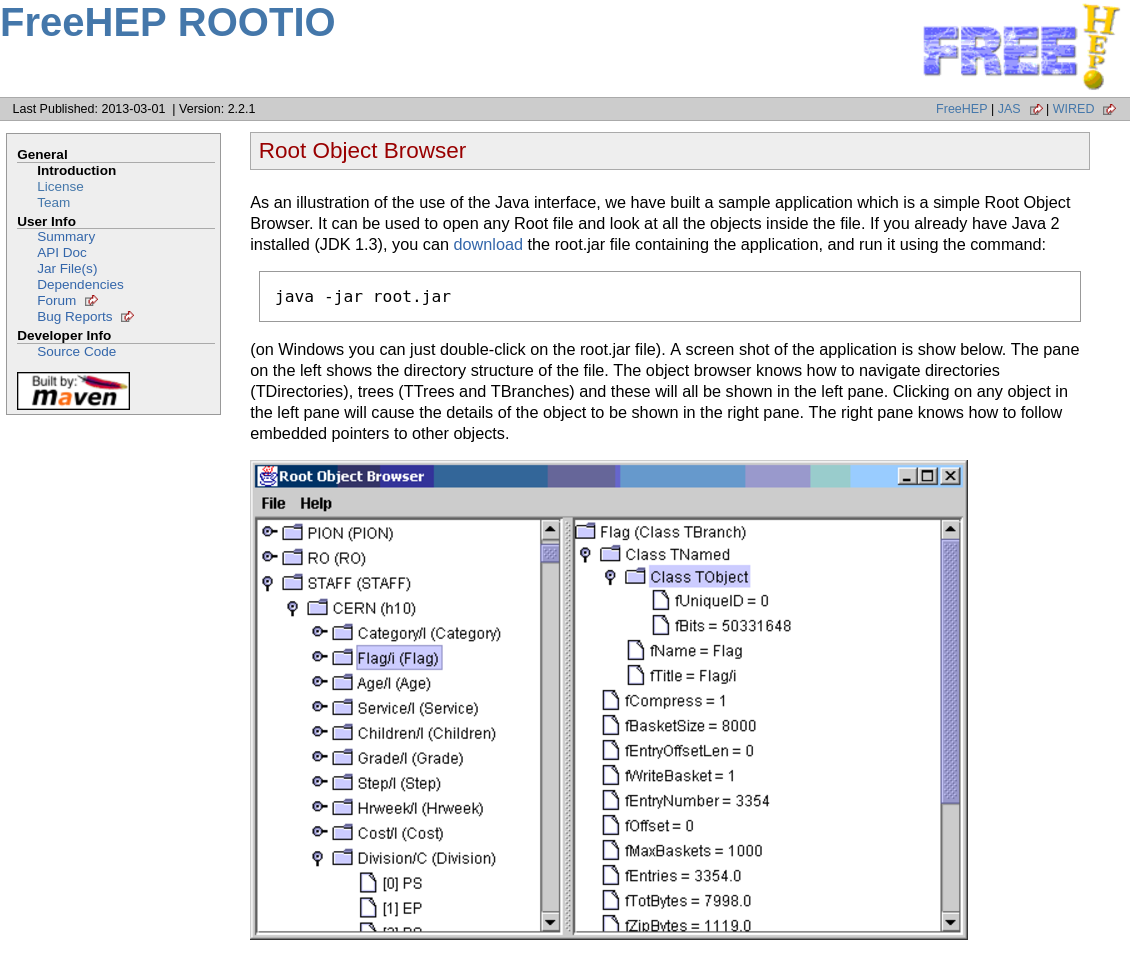
\includegraphics[width=0.9\linewidth]{rootio-screenshot.png}
\end{center}
\end{frame}

\begin{frame}{Pure-Java ROOT reader is old}
\vspace{0.35 cm}
\begin{block}{FreeHEP ROOTIO \scriptsize (\textcolor{blue}{\url{http://java.freehep.org/freehep-rootio/}})}
\vspace{-0.1 cm}
\begin{itemize}
\item Re-implementation of ROOT's I/O in Java.
\item Used as a backend in Java Analysis Studio (JAS).
\item First talks by Tony Johnson in 2001, commits trail off $\sim$2010.
\end{itemize}
\end{block}

\vspace{-0.25 cm}
\begin{uncoverenv}<2->
\begin{block}{Why didn't I consider it an option?}
\vspace{-0.1 cm}
\begin{itemize}
\item Lack of documentation; high-level interface described on website no longer exists.
\item Immediately failed when presented with recent ROOT file.
\item Can't get in touch with Tony Johnson.
\end{itemize}
\end{block}
\end{uncoverenv}

\vspace{-0.25 cm}
\begin{uncoverenv}<3->
\begin{block}{What changed?}
\vspace{-0.1 cm}
\begin{itemize}
\item I tried accessing data in a low-level way.
\item Only 3 minor bug-fixes needed to read modern ROOT files, even a complex CMS AOD!
\end{itemize}
\end{block}
\end{uncoverenv}
\end{frame}

\begin{frame}{Features}
\renewcommand{\arraystretch}{1.5}
\begin{tabular}{p{0.85\linewidth} c}
& \textcolor{red}{verified?} \\
Can read complex structures (directly via TBaskets). & \textcolor{red}{$\surd$} \\
Only small corrections remain. & \textcolor{red}{likely} \\
Well-organized; class/method names mirror ROOT. & \textcolor{red}{$\surd$} \\
JIT-compiles streamers, rather than generic functions. & \textcolor{red}{$\surd$} \\
Can write objects to ROOT files as well. & \\
Has an embedded XRootD client (HDFS and EOS!). & \\
\end{tabular}
\end{frame}

\begin{frame}[fragile]{Project: expose ROOT format in Spark}
\vspace{0.5 cm}
\begin{columns}[t]
\column{0.5\linewidth}
\textcolor{darkblue}{\large \bf root4j}

\vspace{0.1 cm}
\begin{itemize}
\item Fork of original FreeHEP with JAS dependency and GUI components removed.
\item Java, minimal dependencies, built with Maven.
\item LGPL 2.1 (like original).
\end{itemize}

\column{0.5\linewidth}
\textcolor{darkblue}{\large \bf spark-root}

\vspace{0.1 cm}
\begin{itemize}
\item New project, depends on root4j, Hadoop, Spark.
\item Presents ROOT TChain as a Spark DataFrame.
\item Scala, built with SBT.
\item Apache 2.0.
\end{itemize}
\end{columns}
\end{frame}

\begin{frame}[fragile]{Example session (\only<1>{Spark}\only<2>{PySpark})}
\vspace{0.5 cm}
Launch Spark with packages from Maven Central.
\small
\begin{onlyenv}<1>
\begin{minted}{bash}
spark-shell --packages \
    org.diana-hep:spark-root_2.11:x.y.z, \
    org.diana-hep:histogrammar_2.11:1.0.4
\end{minted}
\end{onlyenv}
\begin{onlyenv}<2>
\begin{minted}{bash}
pyspark --packages \
    org.diana-hep:spark-root_2.11:x.y.z, \
    org.diana-hep:histogrammar_2.11:1.0.4
\end{minted}
\end{onlyenv}

\normalsize
Read ROOT file like any other format for a DataFrame.

\small
\begin{onlyenv}<1>
\begin{minted}{scala}
import org.dianahep.sparkroot._
val df = spark.sqlContext.read.root(
             "hdfs://path/to/files/*.root")
\end{minted}
\end{onlyenv}
\begin{onlyenv}<2>
\begin{minted}{python}
df = sqlContext.read \
       .format("org.dianahep.sparkroot") \
       .load("hdfs://path/to/files/*.root")
\end{minted}
\end{onlyenv}

\begin{verbatim}
df.printSchema()
root
 |-- met: float (nullable = false)
 |-- muons: array (nullable = false)
 |    |-- element: struct (containsNull = false)
 |    |    |-- pt: float (nullable = false)
 |    |    |-- eta: float (nullable = false)
 |    |    |-- phi: float (nullable = false)
 |-- jets: array (nullable = false)
\end{verbatim}
\end{frame}

\begin{frame}[fragile]{Example session (\only<1>{Spark}\only<2>{PySpark})}
\small
\begin{verbatim}
df.show()
+---------+--------------------+--------------------+
|      met|               muons|                jets|
+---------+--------------------+--------------------+
| 55.59374|[[28.07075,-1.331...|[[194.19714,-2.65...|
|39.440292|                  []|[[93.64958,-0.273...|
|2.1817229|[[5.523367,-0.375...|[[96.09923,0.7058...|
|  80.5822|[[48.910114,-0.17...|[[165.2686,0.2623...|
| 84.43806|                  []|[[51.87823,1.6442...|
| 84.63146|[[33.84279,-0.062...|[[137.74776,-0.45...|
| 393.8167|[[25.402626,-0.66...|[[481.8268,-1.115...|
|  75.0873|                  []|[[144.62373,-2.21...|
|2.6512942|[[6.851382,2.3145...|[[72.08256,-1.713...|
|36.753353|                  []|[[72.7172,-1.3265...|
+---------+--------------------+--------------------+
only showing top 10 rows
\end{verbatim}
\end{frame}

\begin{frame}[fragile]{Example session (\only<1>{Spark}\only<2>{PySpark})}
\vspace{0.25 cm}
(This is from a real CMS analysis.)

\begin{onlyenv}<1>
\small
\begin{minted}{scala}
// Bring dollar-sign notation into scope.
import spark.sqlContext.implicits._

// Compute event weight with columns and constants.
df.select(($"lumi"*xsec/nGen) * $"LHE_weight"(309))
  .show()

// Pre-defined function (notation's a little weird).
val isGoodEvent = (
    ($"evtHasGoodVtx" === 1) &&
    ($"evtHasTrg" === 1)     &&
    ($"tkmet" >= 25.0)       &&
    ($"Mu_pt" >= 30.0)       &&
    ($"W_mt" >= 30.0))

// Use it.
println("%d events pass".format(
                    df.where(isGoodEvent).count()))
\end{minted}
\end{onlyenv}

\begin{onlyenv}<2>
\small
\begin{minted}{python}
# Python trick: make columns Python variables.
for name in df.schema.names:
    exec("{0} = df['{0}']".format(name))

# Look at a few event weights.
df.select((lumi*xsec/nGen) * LHE_weight[309]).show()

# Pre-defined function (notation's a little different).
isGoodEvent = (
    (evtHasGoodVtx == 1) &
    (evtHasTrg == 1)     &
    (tkmet >= 25.0)      &
    (Mu_pt >= 30.0)      &
    (W_mt >= 30.0))

# Use it.
print "{} events pass".format(
                  df.where(isGoodEvent).count())
\end{minted}
\end{onlyenv}
\end{frame}

\begin{frame}[fragile]{Example session (\only<1>{Spark}\only<2->{PySpark})}
\vspace{0.5 cm}
\small
\begin{onlyenv}<1>
\begin{minted}{scala}
// Use Histogrammar to make histograms.
import org.dianahep.histogrammar._
import org.dianahep.histogrammar.sparksql._
import org.dianahep.histogrammar.bokeh._

// Define histogram functions with SparkSQL Columns.
val h = df.Label(
         "muon pt" -> Bin(100, 0.0, 50.0, $"Mu_pt"),
         "W mt" -> Bin(100, 0.0, 120.0, $"W_mt"))

// Plot the histograms with Bokeh.
val bokehhist = h.get("muon pt").bokeh()
plot(bokehhist)
val bokehhist2 = h.get("W mt").bokeh()
plot(bokehhist2)
\end{minted}
\end{onlyenv}

\begin{onlyenv}<2->
\begin{minted}{python}
# Use Histogrammar to make histograms.
from histogrammar import *
import histogrammar.sparksql
histogrammar.sparksql.addMethods(df)

# Define histogram functions with SparkSQL Columns.
h = df.Label(
      muon_pt = Bin(100, 0.0, 50.0, Mu_pt),
      W_mt = Bin(100, 0.0, 120.0, W_mt))

# Plot the histograms with PyROOT.
roothist = h.get("muon_pt").plot.root("muon pt")
roothist.Draw()
roothist2 = h.get("W_mt").plot.root("W mt")
roothist2.Draw()
\end{minted}
\end{onlyenv}

\vspace{-2 cm}
\begin{uncoverenv}<3>
\mbox{ } \hfill 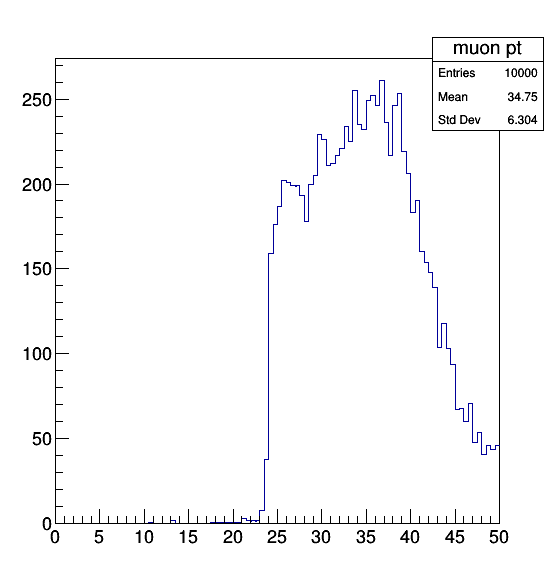
\includegraphics[width=3 cm]{muonpt.png}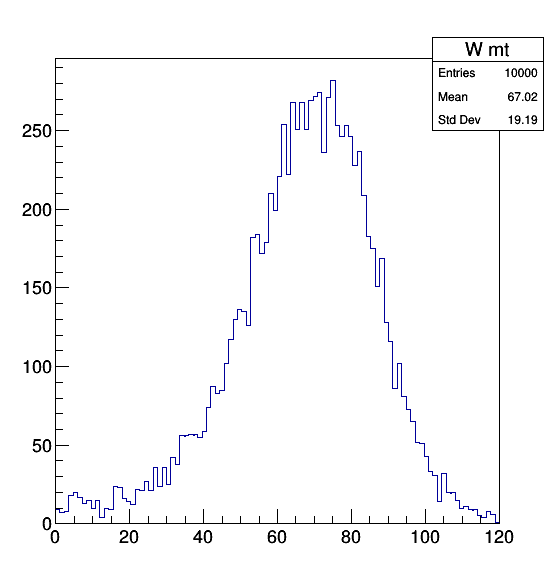
\includegraphics[width=3 cm]{wmt.png}
\end{uncoverenv}
\end{frame}

\begin{frame}{Performance}
\vspace{0.5 cm}
\textcolor{darkblue}{Microbenchmark:} read one nested branch ($\chi^2$ of tracks in events),

\textcolor{white}{Microbenchmark:} lower is better,

\textcolor{white}{Microbenchmark:} best Java (orange) vs best C++ (blue).

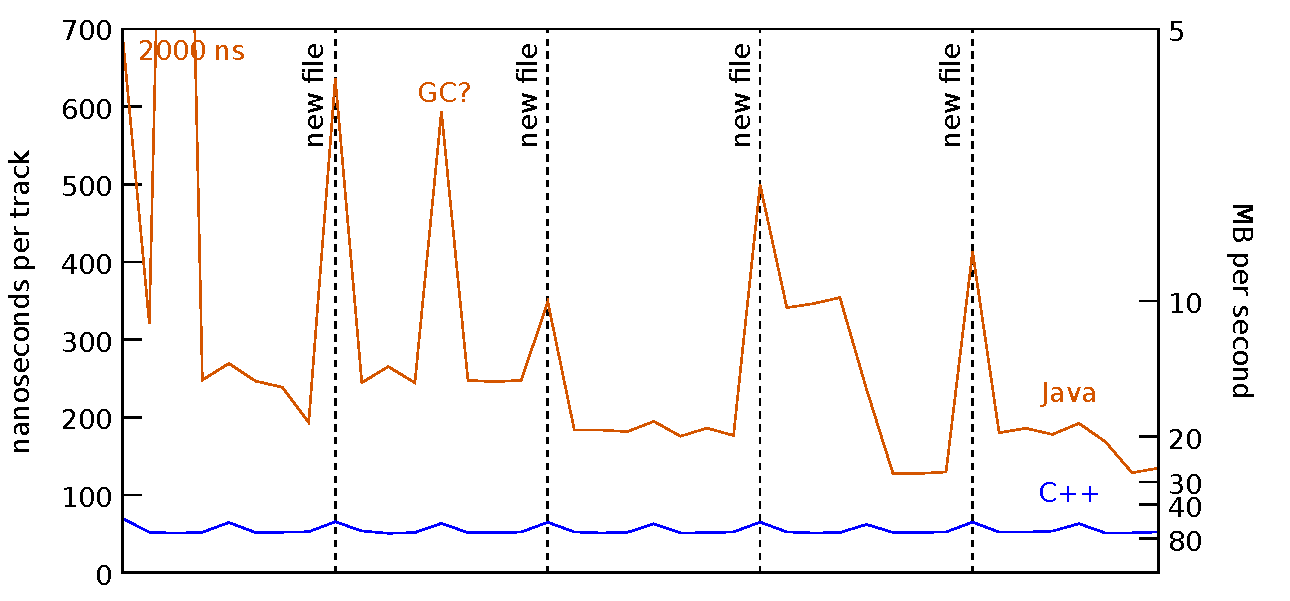
\includegraphics[width=\linewidth]{performance.pdf}

\mbox{ } \hfill time $\longrightarrow$ \hfill \mbox{ }

\vspace{0.15 cm}
\hfill \textcolor{blue}{\tiny (\url{https://gist.github.com/jpivarski/e8b9da99152bccf70ba187cdab149563})\hspace{-0.5 cm}}
\end{frame}

\begin{frame}{Performance}

{\Large However, best performance is not typical.}

\vspace{0.2 cm}
\begin{itemize}
\item My attempt at a C++ reader was 120 times worse than the best-case C++. (I got help from a ROOT expert.)
\item<2-> DataFrame interface only has one way to read; use the best-case Java for that interface.
\item<3-> Spark preemptively caches DataFrames. Access time is highly dependent on history.
\end{itemize}
\end{frame}

\begin{frame}{Performance}
\vspace{0.5 cm}
\begin{itemize}\setlength{\itemsep}{0.4 cm}
\item Spark's data source interface provides information about which columns will be needed and which rows to filter.

\vspace{0.2 cm}
\textcolor{darkblue}{$\rightarrow$ ROOT files are columnar; we can apply these hints.}

\item<2-> RDDs are slow in PySpark because data has to be serialized into Python to execute the Python functions on them.

\vspace{0.2 cm}
DataFrames are fast because PySpark sends the Column expression to the JVM and the JVM calculates it in pure Java.

\vspace{0.2 cm}
\textcolor{darkblue}{$\rightarrow$ Histogrammar-Python now sends Column expressions to be}

\textcolor{white}{$\rightarrow$} \textcolor{darkblue}{computed by Histogrammar-Scala.}

\vspace{0.2 cm}
\textcolor{white}{$\rightarrow$} \textcolor{darkblue}{Python coordinates big, distributed calculations and}

\textcolor{white}{$\rightarrow$} \textcolor{darkblue}{performs small, local ones.}
\end{itemize}
\end{frame}

\begin{frame}{Status and plans}
\vspace{0.25 cm}
\begin{itemize}
\item root4j/spark-root are in early development.
\begin{itemize}
\item \textcolor{blue}{\url{http://github.com/diana-hep/root4j}}
\item \textcolor{blue}{\url{http://github.com/diana-hep/spark-root}}
\end{itemize}

\item Histogrammar is mature; new features shown here are online.
\begin{itemize}
\item \textcolor{blue}{\url{http://histogrammar.org}}
\end{itemize}
\end{itemize}

\vspace{0.25 cm}
\begin{uncoverenv}<2->
\begin{itemize}
\item root4j/spark-root plans:
\begin{enumerate}
\item Generate DataFrame schemas from ROOT streamers.
\item Load chains by glob pattern. Partition at ``cluster'' boundaries.
\item Read ROOT files from HDFS with data locality.
\item Read ROOT files via XRootD, enabling EOS.
\item Test with many complex ROOT file samples.
\item Support {\it writing} to ROOT files (TTrees and histograms).
\end{enumerate}
\end{itemize}
\end{uncoverenv}
\end{frame}

\end{document}
